\documentclass[tikz,border=5pt]{standalone}
\usepackage[UTF8]{ctex}
\usepackage{amsmath,amssymb}
\usetikzlibrary{arrows.meta,calc}
\definecolor{ink}{HTML}{243447}\definecolor{blue}{HTML}{2765A2}
\definecolor{green}{HTML}{3F7D5B}\definecolor{red}{HTML}{B74739}
\tikzset{body/.style={draw=ink,thick},vec/.style={draw=blue,thick,-{Latex}},
guide/.style={gray!60,dashed},dim/.style={ink,{Latex}-{Latex}},
line cap=round,line join=round}
\newcommand{\bubble}[1]{
\shade[ball color=blue!9](0,0)circle(#1);
\draw[body](0,0)circle(#1);
\draw[guide](#1,0)arc(0:180:#1 and {#1*.28});
\draw[blue](#1,0)arc(0:-180:#1 and {#1*.28});}
\begin{document}
\begin{tikzpicture}
\begin{scope}
\bubble{.18}
\node[anchor=north,align=center]at(0,-1.75){$A$\\$a=4.50\,\mu\mathrm m$\\$P_0,T_0$};
\end{scope}
\begin{scope}[shift={(4.5,0)}]
\bubble{1.44}
\draw[dim](0,1.65)--(1.44,1.65)node[midway,above]{$b=36.0\,\mu\mathrm m$};
\node[anchor=north,align=center]at(0,-1.75){$B$\\$V_B=512V_A$\\$T_B=T_0$};
\end{scope}
\begin{scope}[shift={(9,0)}]
\bubble{.18}
\node[anchor=north,align=center]at(0,-1.75){$C$\\$a=4.50\,\mu\mathrm m$\\$T_C=64T_0$};
\end{scope}
\draw[vec](1.05,0)--(2.7,0)node[midway,above]{等温};
\draw[vec](6.3,0)--(7.95,0)node[midway,above]{可逆绝热};
\draw[green,thick,-{Latex}](9,-3.25)--(9,-3.6)--(0,-3.6)--(0,-3.25);
\node[below]at(4.5,-3.6){$C\to A$：等容冷却};
\end{tikzpicture}
\begin{tikzpicture}[x=.7cm,y=.48cm]
\coordinate(A)at(0,0);\coordinate(B)at(6.2383,-6.2383);\coordinate(C)at(0,4.1589);
\draw[vec](-.7,0)--(7.35,0)node[right]{$\ln(V/V_A)$};
\draw[vec](0,-7.25)--(0,5.25)node[above]{$\ln(P/P_0)$};
\draw[blue,thick](A)--(B);
\draw[blue,thick,-{Latex}](2,-2)--(3,-3);
\draw[red,thick](B)--(C);
\draw[red,thick,-{Latex}](4,-2.5078)--(3,-.8411);
\draw[green,thick,-{Latex}](C)--(A);
\draw[guide](B)--(6.2383,0)node[above,text=ink]{$\ln512$};
\draw[guide](B)--(0,-6.2383)node[left,text=ink]{$-\ln512$};
\draw(-.1,4.1589)--(.1,4.1589)node[left=5pt]{$\ln64$};
\foreach\Z/\pos in{A/below left,B/below right,C/above left}
\fill[ink](\Z)circle(.065)node[\pos]{$\Z$};
\node[blue]at(2.65,-5.0){等温};
\node[red]at(4.6,2.3){可逆绝热};
\node[green,left]at(-.2,2){等容};
\node at(3,-8.1){对数坐标面积不代表体积功};
\end{tikzpicture}
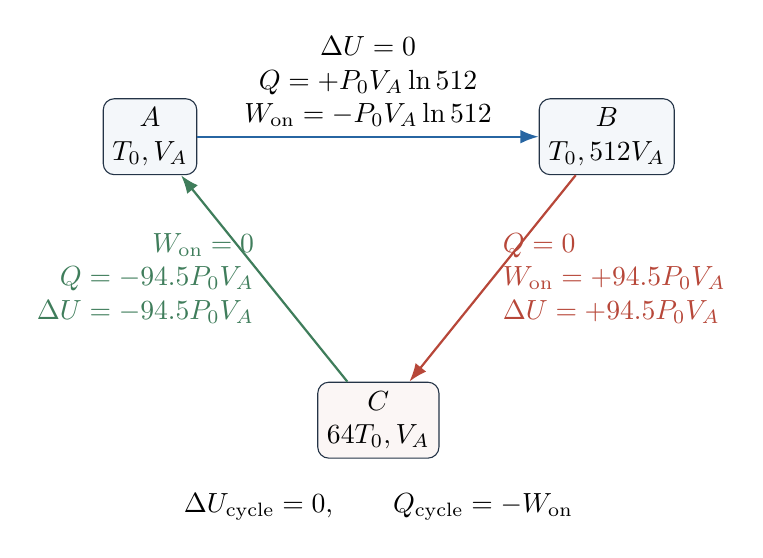
\begin{tikzpicture}
\node[draw=ink,rounded corners,fill=blue!5,align=center] (A)at(0,0){$A$\\$T_0,V_A$};
\node[draw=ink,rounded corners,fill=blue!5,align=center] (B)at(5.8,0){$B$\\$T_0,512V_A$};
\node[draw=ink,rounded corners,fill=red!5,align=center] (C)at(2.9,-3.6){$C$\\$64T_0,V_A$};
\draw[vec](A)--(B)node[midway,above,align=center]{$\Delta U=0$\\$Q=+P_0V_A\ln512$\\$W_{\rm on}=-P_0V_A\ln512$};
\draw[red,thick,-{Latex}](B)--(C)node[midway,right,align=left]{$Q=0$\\$W_{\rm on}=+94.5P_0V_A$\\$\Delta U=+94.5P_0V_A$};
\draw[green,thick,-{Latex}](C)--(A)node[midway,left,align=right]{$W_{\rm on}=0$\\$Q=-94.5P_0V_A$\\$\Delta U=-94.5P_0V_A$};
\node at(2.9,-4.7){$\Delta U_{\rm cycle}=0,\qquad Q_{\rm cycle}=-W_{\rm on}$};
\end{tikzpicture}
\end{document}
